\documentclass[conference]{IEEEtran}
\IEEEoverridecommandlockouts
% The preceding line is only needed to identify funding in the first footnote. If that is unneeded, please comment it out.
\usepackage{cite}
\usepackage{amsmath,amssymb,amsfonts}
\usepackage{algorithmic}
\usepackage{graphicx}
\usepackage{textcomp}
\usepackage{xcolor}
\usepackage{subcaption}

\usepackage{lipsum}% http://ctan.org/pkg/lipsum

\def\BibTeX{{\rm B\kern-.05em{\sc i\kern-.025em b}\kern-.08em
    T\kern-.1667em\lower.7ex\hbox{E}\kern-.125emX}}

\begin{document}

\title{Use Online Dictionary Learning to Get Parts-based Decomposition of Noisy Data}

\author{\IEEEauthorblockN{Daming Lu}
\IEEEauthorblockA{\textit{Baidu Research} \\
Sunnyvale, CA \\
ludaming@baidu.com}
}

\maketitle

\begin{abstract}
A huge amount of data are generated every day.
Extracting interpretable features from the data is becoming
important. Meanwhile, dimension reduction and low-rank approximation
are also becoming important as people want to
factorize big matrix into smaller ones, which are easier to handle.
Sparse coding is such a technique that can factorize a matrix into
sparse linear combinations of basis elements. We found that
through \textit{Online Dictionary Learning}, an efficient sparse coding
algorithm, we could decompose large data matrix with noise
into interpretable dictionary atoms. Such atoms are useful in
reconstructing a denoised data matrix.
\end{abstract}

\begin{IEEEkeywords}
machine learning, sparse coding, online dictionary learning, dimension reduction
\end{IEEEkeywords}

%-%-%-%-%-%-%-%-%-%-%-%-%-%-%-%-%-%-%-%-%-%-%-%-%-%-%-%-%-%-%-%-%-%-%-%
\section{Introduction}
Large amount of high dimensional data are generated every day, thanks to the prosperity of the Internet and big data technology. Due to the difficulty of processing high dimensional data, people intend to factorize or decompose large data matrices into smaller ones. The linear decomposition of a matrix into a few basis elements has been a hot research spot for a long time. At first, general purposed basis matrices were used to represent the large matrix, such as wavelets \cite{b1}. Later, using \textit{ad hoc} matrix learned from specific input data could produce better results. However, although many such decomposition methods could produce smaller matrices, most of these matrices are hardly interpretable, especially when the input data are noisy. Such popular methods include principal component analysis (PCA) \cite{b2}, CUR matrix decomposition \cite{b3}, etc. We found that the \textit{Online Dictionary Learning} method, introduced in \cite{b4}, could not only reduce the matrix dimension, but also get the atoms in the learned dictionary that are interpretable. We applied this technology to two different sets of noisy data and found the extracted atoms very close to the ground truth.

We compared our method with \textit{UoI-NMF\textsubscript{cluster}} \cite{b5} and found our accuracies are better. Meanwhile, we found that \textit{Online Dictionary Learning} runs faster as it does not require the clustering step as in \textit{UoI-NMF\textsubscript{cluster}}. The clustering step is actually crucial for robustness. As a result, \textit{UoI-NMF\textsubscript{cluster}} is more robust compared to \textit{Online Dictionary Learning}, which will be discussed in Section 4. The following sections are organized as below:

\begin{itemize}
\item We first review the core part of \textit{Online Dictionary Learning}.
\item We then introduce the application of \textit{Online Dictionary Learning} on our datasets and compare the results with \textit{UoI-NMF\textsubscript{cluster}}.
\item Finally we discuss potential advantages and disadvantages of both methods.
\end{itemize}

%-%-%-%-%-%-%-%-%-%-%-%-%-%-%-%-%-%-%-%-%-%-%-%-%-%-%-%-%-%-%-%-%-%-%-%
\section{PRELIMINARIES}
\subsection{Online Dictionary Learning}

\textit{Online Dictionary Learning} was first introduced in \cite{b4}. Assume we have a finite training dataset as $ X=[x_1,...x_n] $ in $R^{m\times n}$, we want to learn a dictionary $D$ as a ``good'' representation of signal $x$. Normally the dimension $m$ is relatively small compared to the total amount of data $n$. We want to have a $k\ll n$ such as we can only use a few elements (atoms) in $D$ to represent signal $x$. Our aim is to optimize $\ell(x, D)$ as the $\ell_{1}$ sparse coding problem:
$$ \ell(x, D) \triangleq \min\limits_{\alpha \in R^k} \frac{1}{2}\Arrowvert x-D\alpha \Arrowvert^{2}_{2}+\lambda\Arrowvert \alpha \Arrowvert_{1}$$
where $ \lambda $ is a regularization parameter. This problem is also called \textit{basis pursuit} \cite{b6}, or more commonly, \textit{Lasso}  \cite{b7}. It can be rewritten as a joint optimization problem with respect to the dictionary $D$ and the coefficients $\alpha=[\alpha_1,...,\alpha_n]$ of the
sparse decomposition. Although it is not jointly convex, it can be convex with respect to each of the two variables $D$ and $\alpha$ when
the other one is fixed. An intuitive way of solving this convex optimization problem is to alternatively update one variable with the other one fixed, as proposed in \cite{b8}. In \cite{b9}, it pointed out that instead of minimizing empirical cost, minimizing expected cost is often more demanding. We chose \textit{Online Dictionary Learning} as it does not require explicit learning
rate tuning and is focused on minimizing a local approximations of the expected cost. We followed the algorithm as mentioned in \cite{b4} with a mini-batch extension in order to prevent polluting the initialization.

%-%-%-%-%-%-%-%-%-%-%-%-%-%-%-%-%-%-%-%-%-%-%-%-%-%-%-%-%-%-%-%-%-%-%-%
\section{NUMERIC EXPERIMENTS}
In this section, we illustrate the application of \textit{Online Dictionary Learning} on two datasets: Swimmer dataset and MNIST 2-digit dataset. The details of these two datasets were introduced in \cite{b5}. We used SPAMS library \cite{b10,b11} as our backbone.

%- plot figures -%

%-MNIST-%
\begin{figure*}[!htb]
\centering
\minipage{0.25\textwidth}
  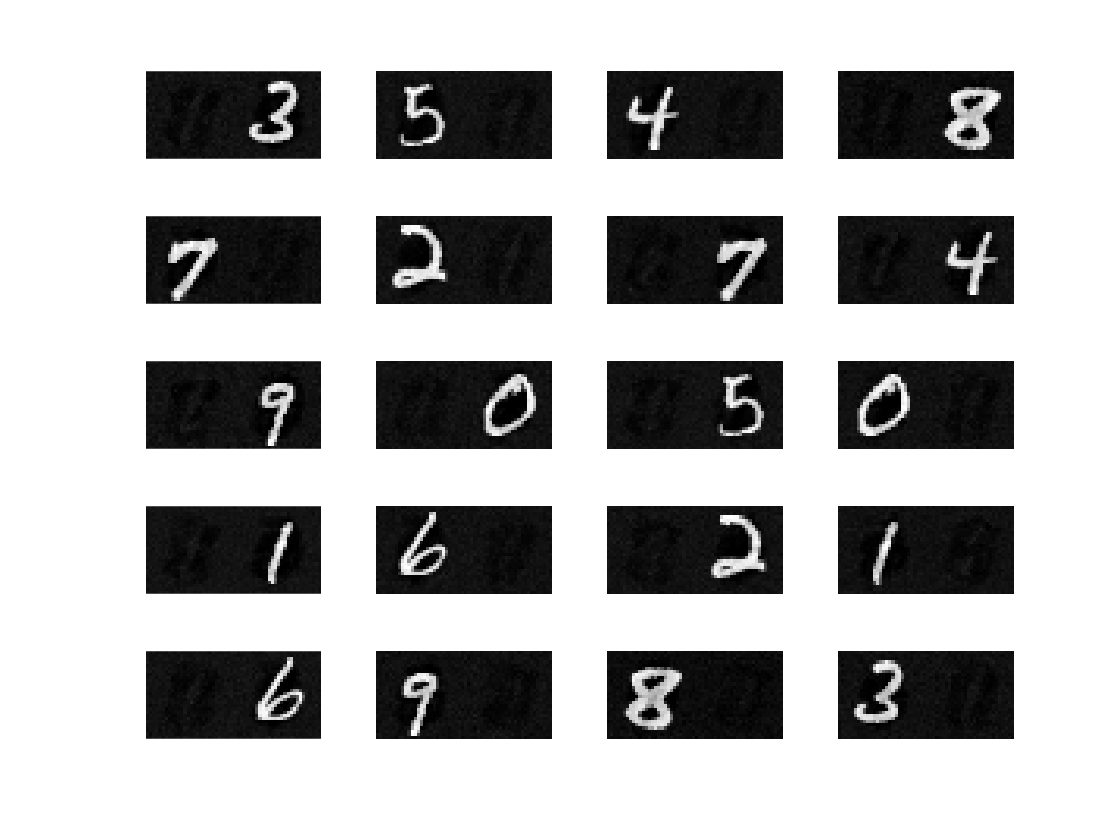
\includegraphics[width=\linewidth]{uoi_best_basis}
\endminipage\hfill
\minipage{0.25\textwidth}
  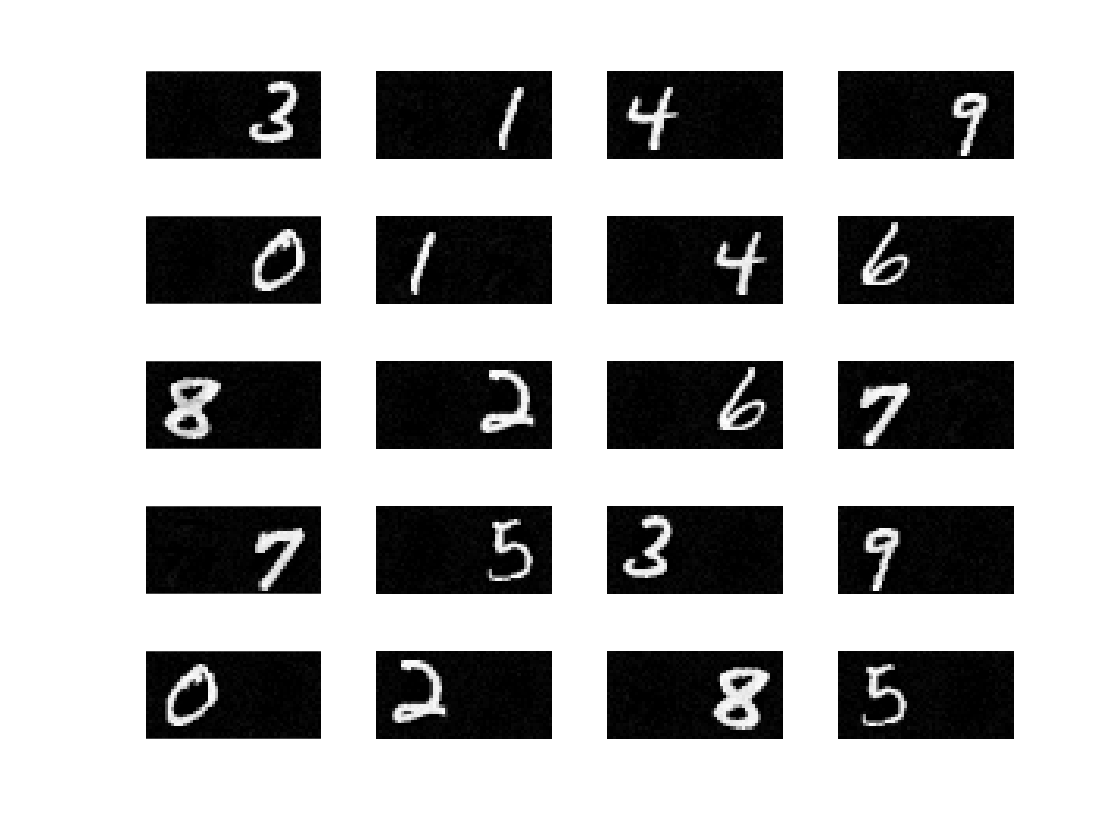
\includegraphics[width=\linewidth]{odl_best_basis_better}
\endminipage\hfill
\minipage{0.25\textwidth}%
  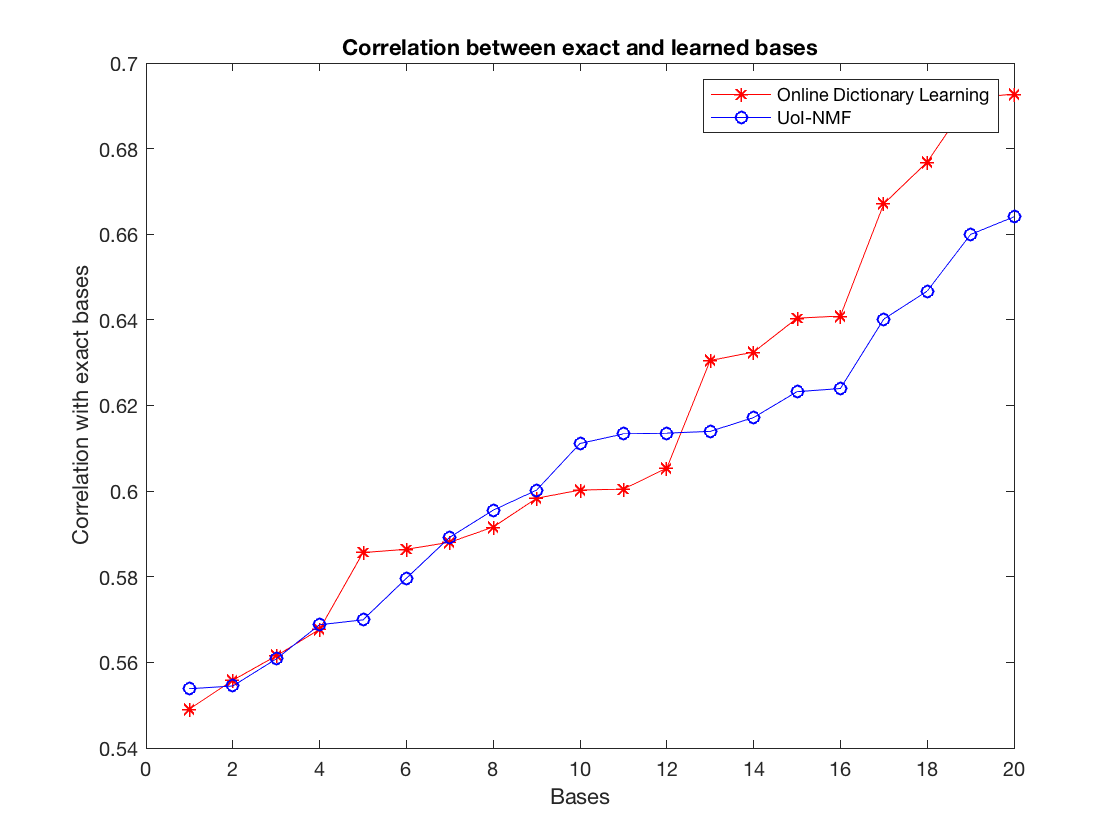
\includegraphics[width=\linewidth]{corr_2in1}
\endminipage
\minipage{0.25\textwidth}%
  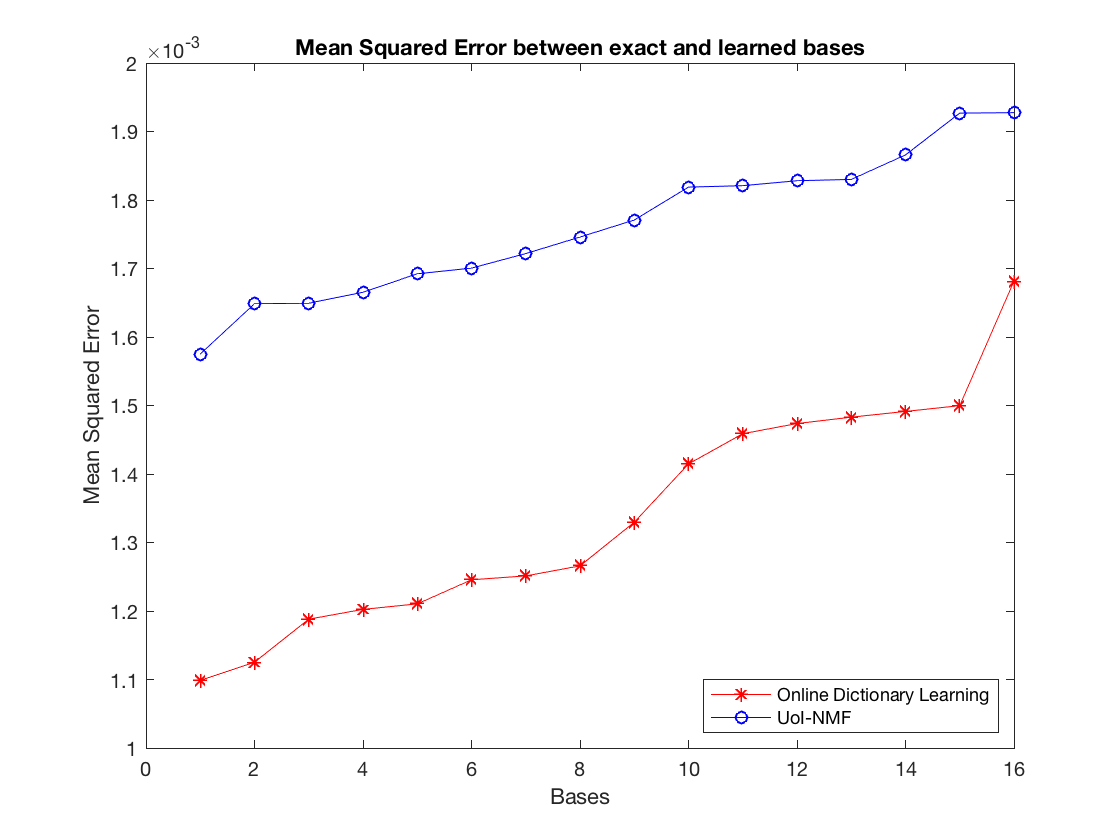
\includegraphics[width=\linewidth]{mse_2in1}
\endminipage
\caption{First $5\times 4$ images: 20 bases learned by \textit{UoI-NMF\textsubscript{cluster}} for the high noise MNIST two digits data. Second $5\times 4$ images: 20 bases learned by \textit{Online Dictionary Learning} for the same dataset. Third figure: Correlation between exact and learned bases for \textit{UoI-NMF\textsubscript{cluster}} and \textit{Online Dictionary Learning}. Fourth figure: Mean Squared Error between exact and learned bases for \textit{UoI-NMF\textsubscript{cluster}} and \textit{Online Dictionary Learning}. }\label{fig:mnist_4}
\end{figure*}

%-Swimmer-%
\begin{figure*}[!htb]
\centering
\minipage{0.25\textwidth}
  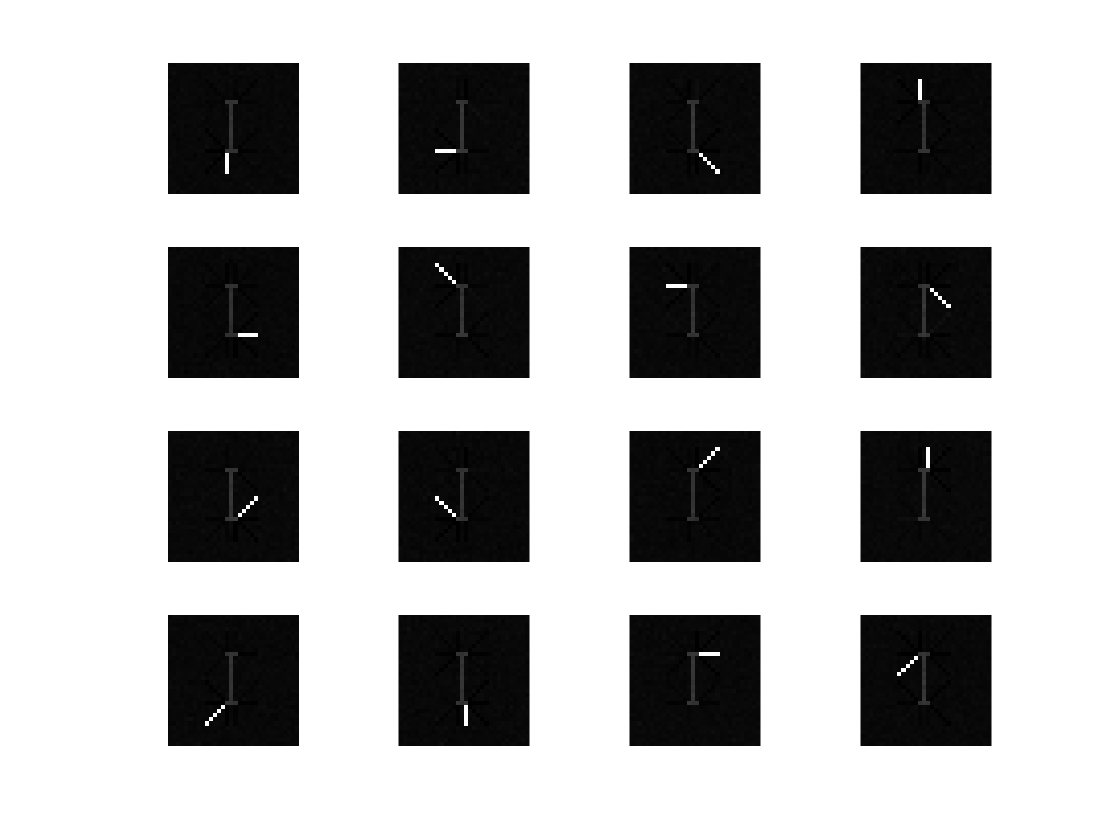
\includegraphics[width=\linewidth]{swimmer_uoi_best_basis}
\endminipage\hfill
\minipage{0.25\textwidth}
  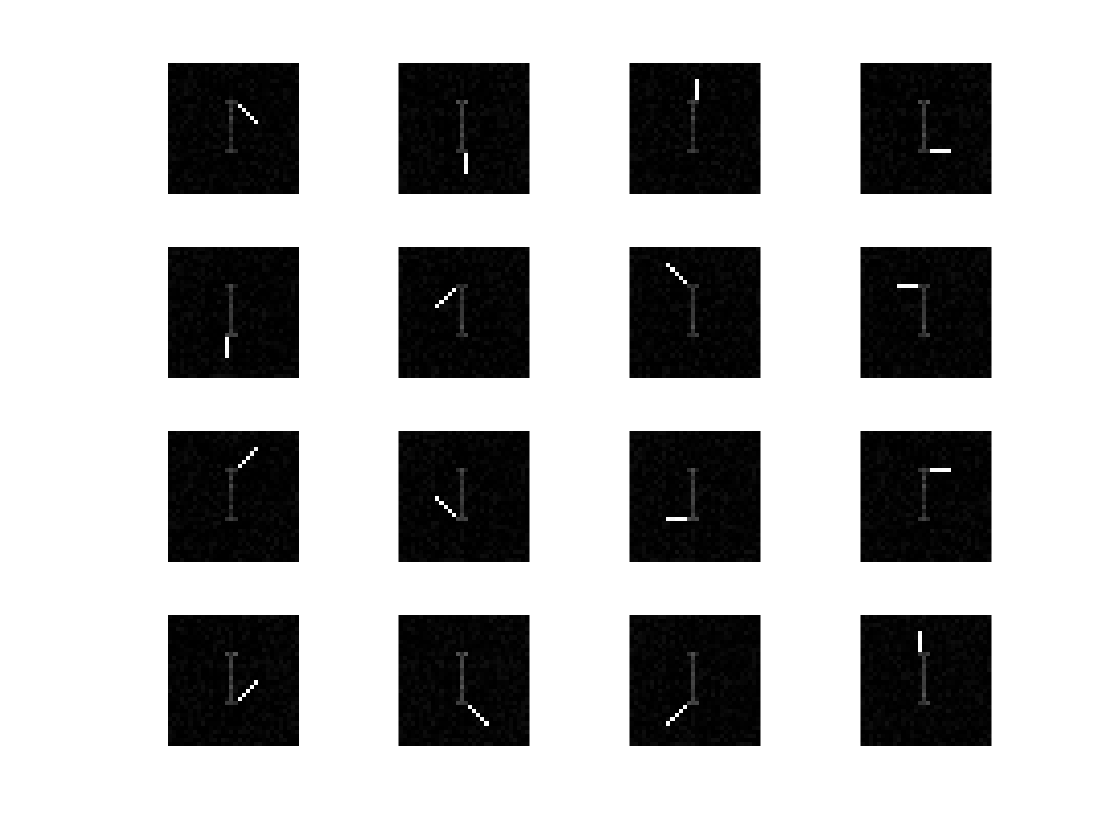
\includegraphics[width=\linewidth]{swimmer_odl_best_641}
\endminipage\hfill
\minipage{0.25\textwidth}%
  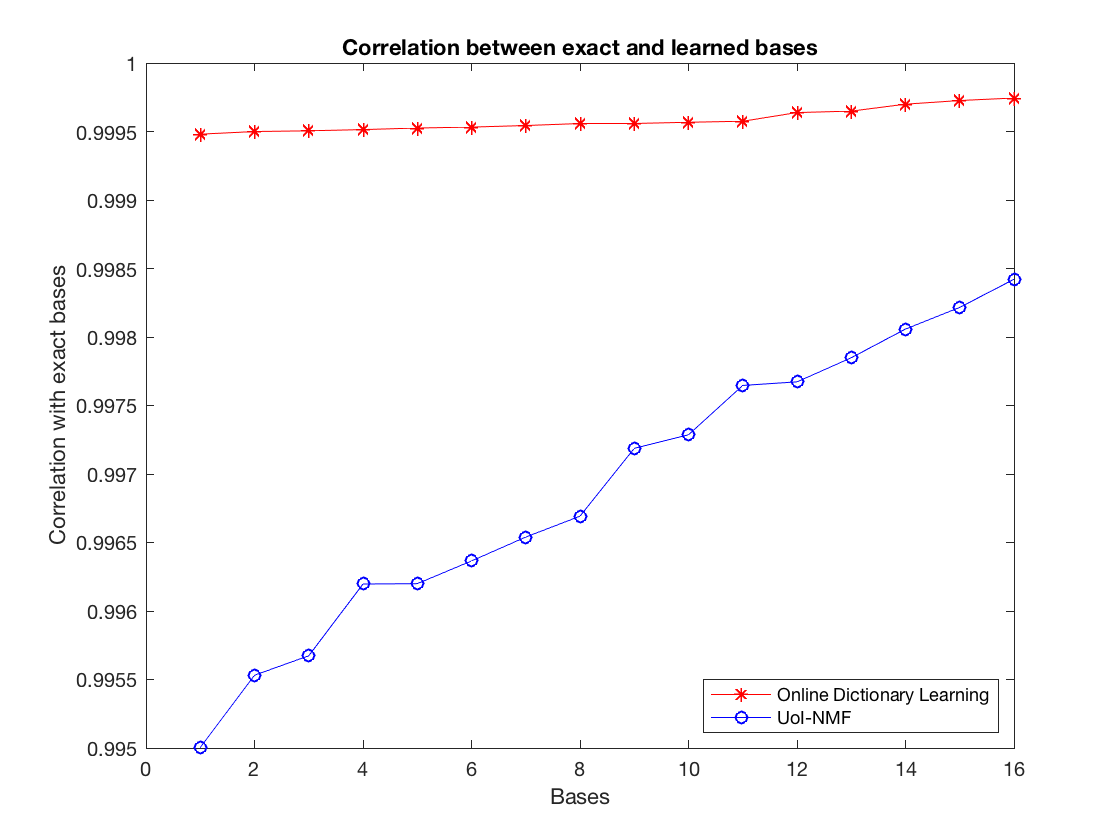
\includegraphics[width=\linewidth]{swimmer_corr_2in1}
\endminipage
\minipage{0.25\textwidth}%
  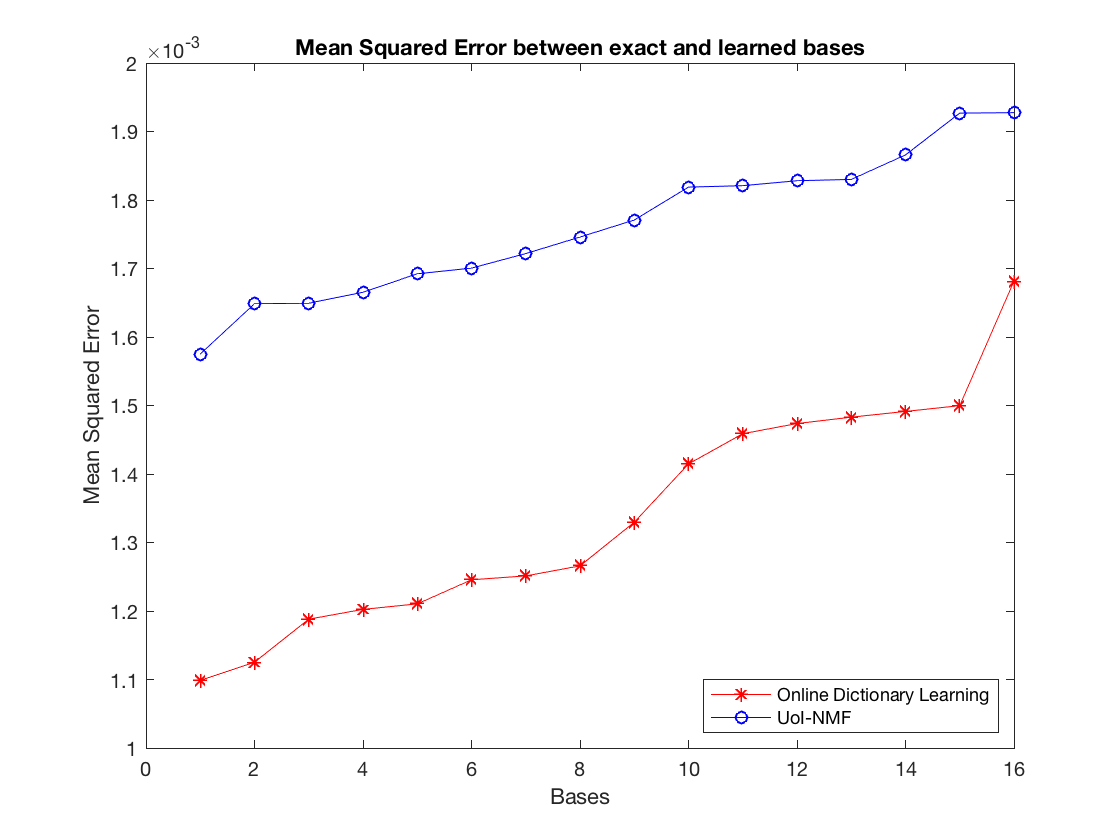
\includegraphics[width=\linewidth]{swimmer_mse_2in1}
\endminipage
\caption{First $4\times 4$ images: 16 bases learned by \textit{UoI-NMF\textsubscript{cluster}} for the
high noise Swimmer data. Second $4\times 4$ images: 16 bases learned by \textit{Online Dictionary Learning} for the same dataset. Third figure: Correlation between exact and learned bases for \textit{UoI-NMF\textsubscript{cluster}} and \textit{Online Dictionary Learning}. Fourth figure: Mean Squared Error between exact and learned bases for \textit{UoI-NMF\textsubscript{cluster}} and \textit{Online Dictionary Learning}. }\label{fig:swimmer_4}
\end{figure*}

%-%-%-%-%-%-%-%-%-%-%-%-%-%-%-%-%-%-%-%-%-%-%-%-%-%-%-%-%-%-%-%-%-%-%-%
After 1,000 iterations, the performance metrics as well as the learned atoms are shown in Fig. 1 for MNIST 2-digits dataset, side by side with \textit{UoI-NMF\textsubscript{cluster}}. The corresponding results for Swimmer dataset are shown in Fig. 2.

We can tell from the metrics that \textit{Online Dictionary Learning} has a slightly better accuracy than \textit{UoI-NMF\textsubscript{cluster}}. Both methods learned the bases/parts pretty well. Moreover, since \textit{Online Dictionary Learning} does not have the clustering part as in \textit{UoI-NMF\textsubscript{cluster}}, it runs faster, as is shown in Table. I.

\begin{table}[htbp]
\caption{Time Cost of the Two Methods}
\begin{center}
\begin{tabular}{|c|c|c|}
\hline
\textbf{Dataset}&\multicolumn{2}{|c|}{\textbf{Time Cost (sec)}} \\
\cline{2-3}
 & \textbf{\textit{UoI-NMF\textsubscript{cluster}}}& \textbf{\textit{Online Dictionary Learning}} \\
\hline
MNIST 2-digits & 112.46 & 1.89 \\
\hline
Swimmer & 213.82 & 2.29 \\
\hline
\end{tabular}
\label{tab1}
\end{center}
\end{table}

A large amount of time used by \textit{UoI-NMF\textsubscript{cluster}} is spent on clustering to get strong signal on the bases, which means \textit{UoI-NMF\textsubscript{cluster}} is more robust. Table. II \& III endorse this conclusion by showing reconstruction errors of the two methods with noisy and original data. We can see that both methods have similar reconstruction errors on noisy data. But \textit{UoI-NMF\textsubscript{cluster}} has a much lower reconstruction error on original data. We consider it as a benefit of the stronger bases learned by \textit{UoI-NMF\textsubscript{cluster}}. We also observed that in multiple runs, \textit{UoI-NMF\textsubscript{cluster}} inclines to give stable results of good quality whereas \textit{Online Dictionary Learning} could occasionally get polluted by the noise and get poor results.

\begin{table}[htbp]
\caption{Reconstruction Error with Noisy Data}
\begin{center}
\begin{tabular}{|c|c|c|}
\hline
\textbf{Dataset}&\multicolumn{2}{|c|}{\textbf{Reconstruction Error}} \\
\cline{2-3}
 & \textbf{\textit{UoI-NMF\textsubscript{cluster}}}& \textbf{\textit{Online Dictionary Learning}} \\
\hline
MNIST 2-digits & 192.9003 & 195.2450 \\
\hline
Swimmer & 242.0457 & 274.0686 \\
\hline
\end{tabular}
\label{tab2}
\end{center}
\end{table}

\begin{table}[htbp]
\caption{Reconstruction Error with Original Data}
\begin{center}
\begin{tabular}{|c|c|c|}
\hline
\textbf{Dataset}&\multicolumn{2}{|c|}{\textbf{Reconstruction Error}} \\
\cline{2-3}
 & \textbf{\textit{UoI-NMF\textsubscript{cluster}}}& \textbf{\textit{Online Dictionary Learning}} \\
\hline
MNIST 2-digits & 44.7821 & 238.2057 \\
\hline
Swimmer & 57.4769 & 261.9353 \\
\hline
\end{tabular}
\label{tab3}
\end{center}
\end{table}

\section{CONCLUSION}

We proposed a new application of \textit{Online Dictionary Learning} to the task of parts-based decomposition of noisy data in two datasets and compared the performance with the state-of-the-art method \textit{UoI-NMF\textsubscript{cluster}}. We found that both methods could find the actual bases in the process of dimension reduction for noisy data. \textit{UoI-NMF\textsubscript{cluster}} takes longer time, mainly due to the DBSCAN clustering step. However, we found this step crucial for the robustness. The clustering step indeed consolidated the learned bases so that they are more robust to noise. \textit{Online Dictionary Learning}, on the other hand, runs faster and has the potential of dealing with large amount of data, in an online or streaming way. In \cite{b12}, it shows that both methods share the same mathematical foundation. That is why both could find the parts-based components.

\section{ACKNOWLEDGMENT}

The author would like to thank Shashanka Ubaru for providing thought-provoking ideas about sparse coding, dictionary learning and non-convex optimization.

\begin{thebibliography}{00}

\bibitem{b1} Mallat, S, ``A wavelet tour of signal processing'' 2nd ed., Academic Press, New York 1999.

\bibitem{b2} Abdi H, Williams LJ. Principal component analysis. Wiley interdisciplinary reviews: computational statistics. 2010 Jul;2(4):433-59.

\bibitem{b3} Mahoney MW, Drineas P. CUR matrix decompositions for improved data analysis. Proceedings of the National Academy of Sciences. 2009 Jan 10:pnas-0803205106.

\bibitem{b4} Mairal J, Bach F, Ponce J, Sapiro G. Online dictionary learning for sparse coding. InProceedings of the 26th annual international conference on machine learning 2009 Jun 14 (pp. 689-696). ACM.


\bibitem{b5} Ubaru S, Wu K, Bouchard KE. UoI-NMFcluster: A Robust Nonnegative Matrix Factorization Algorithm for Improved Parts-Based Decomposition and Reconstruction of Noisy Data. InMachine Learning and Applications (ICMLA), 2017 16th IEEE International Conference on 2017 Oct 3 (pp. 241-248). IEEE.

\bibitem{b6} Chen SS, Donoho DL, Saunders MA. Atomic decomposition by basis pursuit. SIAM review. 2001;43(1):129-59.

\bibitem{b7} Tibshirani R. Regression shrinkage and selection via the lasso. Journal of the Royal Statistical Society. Series B (Methodological). 1996 Jan 1:267-88.

\bibitem{b8} Lee H, Battle A, Raina R, Ng AY. Efficient sparse coding algorithms. InAdvances in neural information processing systems 2007 (pp. 801-808).

\bibitem{b9} Bottou L, Bousquet O. The tradeoffs of large scale learning. InAdvances in neural information processing systems 2008 (pp. 161-168).

\bibitem{b10} Mairal J, Bach F, Ponce J, Sapiro G. Online learning for matrix factorization and sparse coding. Journal of Machine Learning Research. 2010;11(Jan):19-60.

\bibitem{b11} Mairal J, Bach F, Ponce J, Sapiro G. Online dictionary learning for sparse coding. InProceedings of the 26th annual international conference on machine learning 2009 Jun 14 (pp. 689-696). ACM.

\bibitem{b12} Donoho D, Stodden V. When does non-negative matrix factorization give a correct decomposition into parts?. InAdvances in neural information processing systems 2004 (pp. 1141-1148).

\end{thebibliography}
\vspace{12pt}


\end{document}
